%%%%%%%%%%%%%%%%%%%%%%%%%%%%%%%%%%%%%%%%%
% University/School Laboratory Report
% LaTeX Template
% Version 3.1 (25/3/14)
%
% This template has been downloaded from:
% http://www.LaTeXTemplates.com
%
% Original author:
% Linux and Unix Users Group at Virginia Tech Wiki 
% (https://vtluug.org/wiki/Example_LaTeX_chem_lab_report)
%
% License:
% CC BY-NC-SA 3.0 (http://creativecommons.org/licenses/by-nc-sa/3.0/)
%
%%%%%%%%%%%%%%%%%%%%%%%%%%%%%%%%%%%%%%%%%

%----------------------------------------------------------------------------------------
%	PACKAGES AND DOCUMENT CONFIGURATIONS
%----------------------------------------------------------------------------------------

\documentclass{article}


\usepackage{siunitx} % Provides the \SI{}{} and \si{} command for typesetting SI units
\usepackage{graphicx} % Required for the inclusion of images
\usepackage{amsmath} % Required for some math elements 
\usepackage{url}
\usepackage{algorithm}
\usepackage{algpseudocode}
\usepackage{amsmath}
\usepackage{graphics}
\usepackage{epsfig}
\usepackage{indentfirst}
\usepackage{textcomp}
%\usepackage[showframe=true]{geometry}
\usepackage{geometry}
\usepackage{changepage}
\usepackage[flushleft]{threeparttable}
\usepackage{graphicx}




\renewcommand{\labelenumi}{\alph{enumi}.} % Make numbering in the enumerate environment by letter rather than number (e.g. section 6)

\newcounter{algsubstate}
\renewcommand{\thealgsubstate}{\alph{algsubstate}}
\newenvironment{algsubstates}
{\setcounter{algsubstate}{0}%
	\renewcommand{\State}{%
		\stepcounter{algsubstate}%
		\Statex {\footnotesize\thealgsubstate:}\space}}
{}


\newenvironment{itquote}
{\begin{quote}\itshape}
	{\end{quote}\ignorespacesafterend}
\newenvironment{itpars}
{\par\itshape}
{\par}



%\usepackage{times} % Uncomment to use the Times New Roman font

%----------------------------------------------------------------------------------------
%	DOCUMENT INFORMATION
%----------------------------------------------------------------------------------------

\title{ Reconstructing collapsed complex network to find most influential nodes  } % Title

\author{Fengkuangtian \textsc{Zhu}} % Author name

\begin{document}
	
	\maketitle % Insert the title, author and date
	
	
	
	\begin{center}
		\begin{tabular}{c}
			Solution of Datacastle Master Competition	\\
			Team ID: zhfkt 
		\end{tabular}
	\end{center}
	
	% If you wish to include an abstract, uncomment the lines below
	\begin{abstract}
		This solution paper is to demonstrate the solution of algorithm in identifying vital nodes in complex networks for Datacastle Master Competition . Compared with traditional algorithms including Betweenness\cite{wikiBetweennesscentrality}, Closeness\cite{wikiClosenesscentrality}, PageRank\cite{wikiPageRank}, Degree\cite{wikiCentrality} and Collective Influence\cite{morone2015influence}\cite{morone2016collective}, the new proposed algorithm of reconstructing collapsed complex network to find most influential nodes is able to achieve the better performance on the 8 competition datasets in terms of robustness\cite{schneider2011mitigation} and speed. The new implementation by c++ of the popular algorithm Collective Influence (CI) is introduced as well. All code in the paper can be found at the link https://github.com/zhfkt/ComplexCi \cite{zhfktgithub} \cite{zhfkt2017887989}
	\end{abstract}
	
	%----------------------------------------------------------------------------------------
	%	SECTION 1
	%----------------------------------------------------------------------------------------
	
	\section{DataCastle Master Competition background}
	
	From \cite{masterCompetitionbackground} , the detail of the Master Competition background held by DataCastle is described below:
	
	\begin{itquote}
		
		Disparate networks, including social networks, communication networks and biological networks, are playing an increasingly important role on natural and social-economic systems. A core problem, therein, is to measure the significance of individual nodes. For instance, a super spreader in HongKong triggered transmission of SARS to a significantly greater number of other people than 100 normal infected persons; a rumour re-tweeted by a celebrity may spread much broader than that by an obscure person.
		
		Therefore it is necessary to develop a method to identify the virulence genes in large-scale gene regulatory networks, to find the super-spreaders in large-scale social networks, and to detect the key enterprises with serious systematic financial risk in large-scale financial networks.
		
		Those tasks could be formalized as a generic challenge that is identifying vital nodes in networks that are important for sustaining connectivity. This challenge, aka optimal percolation, is a well-documented issue in network science. With great anticipation of making big progress on this problem, we successfully invited some experts and hope the great participants will create novel and effective solutions.  		
	\end{itquote}

	
	The competition provides 4 real networks from different fields, including autonomous system network, Internet network, road network and social network, and 4 classical artificial networks as well (total 8 datasets). The numbers of nodes of these networks range from 0.7 million to 2 million. All of them are considered as undirected networks. Table \ref{tab:table1} shows the network name and corresponding numbers of nodes.
	

\begin{table}[]
	
	\centering
	\caption{ Network name and corresponding numbers of nodes}
	\label{tab:table1}
	%\begin{adjustwidth}{0.0cm}{}
		\begin{tabular}{|c|c|c|c|c|c|c|c|c|}
			\hline
			\textbf{Network} & \textbf{model1} & \textbf{model2} & \textbf{model3} & \textbf{model4} & \textbf{real1} & \textbf{real2} & \textbf{real3} & \textbf{real4} \\ \hline
			\textbf{Number} & 1039722         & 1083568         & 997663          & 1001733         & 1694616        & 1957027        & 426485         & 855802         \\ \hline
		\end{tabular}
	%\end{adjustwidth}
	\end{table}

	\section{Introduction}


	Overall, the target of finding most influential nodes algorithm is to give a ranking list of nodes according to their importance. The top-ranked nodes will have more importance. We can remove the nodes from the top-ranked ones in the ranking list generated by algorithm and calculate the size of giant component after each removal, which will break down the network into many disconnected pieces. The ratio of giant component will reach zero with the one-by-one removal operation finally. Therefore, the better algorithm, the sooner the network will collapse to the zero giant component with smaller count of provided nodes. Robustness \cite{schneider2011mitigation} is introduced in the Competition to quantify the performance of ranking nodes methods. 
	
	There are several traditional algorithms such as  Betweenness\cite{wikiBetweennesscentrality}, Closeness\cite{wikiClosenesscentrality}, PageRank\cite{wikiPageRank}, Degree\cite{wikiCentrality} and Collective Influence\cite{morone2015influence}\cite{morone2016collective} for the target. In this paper, the new algorithm is proposed for reconstructing collapsed complex network in order to find most influential nodes. Compared with the traditional algorithms, the new method is able to achieve the better performance in terms of robustness and speed. 
	
	This solution paper will be organized as follows. First, several traditional algorithms will be used to investigate the performance of 8 competition datasets as comparative algorithms. Next, the new reconstructing algorithm will be introduced and verified on datesets in performance. The verification will also include the process of searching parameters for the best result. Lastly, the conclusion will be given. All code in this paper can be found at the link https://github.com/zhfkt/ComplexCi \cite{zhfktgithub} \cite{zhfkt2017887989}

	\section{Experiments on the current algorithms}
	
	In this section, tradition algorithms of Betweenness\cite{wikiBetweennesscentrality}, Closeness\cite{wikiClosenesscentrality}, Degree\cite{wikiCentrality}, PageRank\cite{wikiPageRank} and Collective Influence\cite{morone2015influence}\cite{morone2016collective} will be verified on 8 Datacastle datasets .


	\subsection{Betweenness}
	
	Betweenness is a centrality measure of a vertex within a graph . Betweenness centrality quantifies the number of times a node acts as a bridge along the shortest path between two other nodes \cite{wikiBetweennesscentrality}\cite{freeman1977set}. Here betweenness is used to find the most influential nodes in the complex networks. Robustness value after applying Betweenness on 8 competition datasets is shown in the Table \ref{tab:table2}
	
	
\begin{table}[]
	\begin{adjustwidth}{-1.3cm}{}		
		\begin{threeparttable}
			\centering
			\caption{Robustness value and time after applying Betweenness on 8 competition datasets}
			\label{tab:table2}
		
			\begin{tabular}{|c|c|c|c|c|c|c|c|c|c|}
				\hline
				\textbf{Network}          & \textbf{model1} & \textbf{model2} & \textbf{model3} & \textbf{model4} & \textbf{real1} & \textbf{real2} & \textbf{real3} & \textbf{real4} & \textbf{Total} \\ \hline
				\textbf{Robustness Score} & 0.3125          & 0.2678          & 0.4484          & 0.1952          & 0.1101         & 0.0064         & 0.1582         & 0.1076         & 1.6060         \\ \hline
				\textbf{Time}     & 201733s          & 187508s          & 270524s          & 231936s         & 624256s         & 327145s         & 109726s         & 109685s         & 2062513s        \\ \hline
			\end{tabular}
				\begin{tablenotes}
					\small
					\item\textit{8 datasets are all verified in parallel supported by GraphTools \cite{peixotographtool2014} on the 4-core CPU machine (Intel Xeon E5-2667v4 Broadwell 3.2 GHz).}
				\end{tablenotes}			
	 	\end{threeparttable}
	\end{adjustwidth}
\end{table}
	
	
	Although Betweenness is supported to be executed in utilizing all CPU cores in parallel by GraphTools \cite{peixotographtool2014} to boost , it is still obvious that Betweenness spends nearly 24 days $\simeq$ 1 month in completing the verification of 8 datasets. Considered the time and effort , robustness value of Betweenness is not very well. Betweenness fails to process the networks of million scale to find most influential nodes.
	
	\subsection{Closeness}	
	
	
	In a connected graph, the Closeness centrality of a node is the average length of the shortest path between the node and all other nodes in the graph. Thus the more central a node is, the closer it is to all other nodes \cite{wikiClosenesscentrality}\cite{bavelas1950communication} . Here closeness is also used to find the most influential nodes in the complex networks. Robustness value after applying Closeness on 8 competition datasets is shown in the Table \ref{tab:table3}
	
	\begin{table}[]
		\begin{adjustwidth}{-1.3cm}{}		
			\begin{threeparttable}
				\centering
				\caption{Robustness value and time after applying Closeness on 8 competition datasets}
				\label{tab:table3}
				
				\begin{tabular}{|c|c|c|c|c|c|c|c|c|c|}
					\hline
					\textbf{Network}          & \textbf{model1} & \textbf{model2} & \textbf{model3} & \textbf{model4} & \textbf{real1} & \textbf{real2} & \textbf{real3} & \textbf{real4} & \textbf{Total} \\ \hline
					\textbf{Robustness Score} & 0.4140          & 0.3765          & 0.4624          & 0.3717          & 0.2495         & 0.4454         & 0.2738         & 0.2868         & 2.8801         \\ \hline
					\textbf{Time}     & 63095s           & 63552s           & 71382s           & 46107s           & 136945s         & 161397s         & 17992s          & 31564s          & 592034s         \\ \hline								
				\end{tabular}
				\begin{tablenotes}
					\small
					\item\textit{8 datasets are all verified in parallel supported by GraphTools \cite{peixotographtool2014} on the 8-core CPU machine (Intel Xeon E5-2667v4 Broadwell 3.2 GHz). Please notice that CPU cores in verifying Closeness are 8 cores, double than above CPU cores of machine in \ref{tab:table2} verifying Betweenness}
				\end{tablenotes}			
			\end{threeparttable}
		\end{adjustwidth}
	\end{table}
	
	Similar with Betweenness , although Closeness algorithm is supported to be executed in utilizing all CPU cores in parallel by GraphTools to boost , it is still obvious that Closeness spends nearly 7 days $\simeq$ 1 week in completing the verification of 8 datasets. Considered the time and effort , robustness value of Closeness is also not very well. Closeness fails to process the networks of million scale to find most influential nodes as Betweenness .
	
	
	\subsection{PageRank}	
	
	
	PageRank works by counting the number and quality of links to a page to determine a rough estimate of how important the website is. The underlying assumption is that more important websites are likely to receive more links from other websites \cite{wikiPageRank}\cite{page1999pagerank}. Here PageRank is also used to find the most influential nodes in the complex networks. Robustness value after applying PageRank on 8 competition datasets is shown in the table \ref{tab:table4}
	
	\begin{table}[]
	\begin{adjustwidth}{-1.3cm}{}		
		\begin{threeparttable}
			\centering
			\caption{Robustness value and time after applying PageRank on 8 competition datasets}
			\label{tab:table4}
			
			\begin{tabular}{|c|c|c|c|c|c|c|c|c|c|}
				\hline
				\textbf{Network}          & \textbf{model1} & \textbf{model2} & \textbf{model3} & \textbf{model4} & \textbf{real1} & \textbf{real2} & \textbf{real3} & \textbf{real4} & \textbf{Total} \\ \hline
				\textbf{Robustness Score} & 0.2435          & 0.2043          & 0.4267          & 0.1469          & 0.0522         & 0.1364         & 0.1430         & 0.0832         & 1.436          \\ \hline
				\textbf{Time}     & 701s             & 686s             & 750s             & 552s             & 2106s           & 1845s           & 918s            & 663s            & 8221s           \\ \hline							
			\end{tabular}
			\begin{tablenotes}
				\small
				\item\textit{8 datasets are all verified in single thread supported by GraphTools \cite{peixotographtool2014} on the 4-core CPU (Intel Xeon E5-2667v4 Broadwell 3.2 GHz).}
			\end{tablenotes}			
		\end{threeparttable}
	\end{adjustwidth}
	\end{table}

		
	Compared with Betweenness and Closeness , algorithm PageRank gets much better result in robustness and speed. Especially , PageRank just runs in single thread and uses less resources than betweenness and closeness. Robustness value of PageRank is 1.436 and also better than Betweenness and Closeness 
	
	\subsection{Degree}		

	Historically first and conceptually simplest is degree centrality, which is defined as the number of links incident upon a node . i.e. the number of ties that a node has \cite{wikiCentrality}. The nodes are ranked by degree, and sequentially removed starting from the node of highest degree. The concept of High Degree Adaptive (HDA) is purposed in the \cite{morone2015influence} as a better strategy which is a slightly different from the original Degree algorithm. Degree of the remaining nodes in the adaptive version will be recomputed after each node removal. HDA is used here to find the most influential nodes in the complex networks. Robustness value after applying HDA on 8 competition datasets is shown in the table \ref{tab:table5}
	

		
	\begin{table}[]
		\begin{adjustwidth}{-1.3cm}{}		
			\begin{threeparttable}
				\centering
				\caption{Robustness value and time after applying HDA on 8 competition datasets}
				\label{tab:table5}
				
				\begin{tabular}{|c|c|c|c|c|c|c|c|c|c|}
					\hline
					\textbf{Network}          & \textbf{model1} & \textbf{model2} & \textbf{model3} & \textbf{model4} & \textbf{real1} & \textbf{real2} & \textbf{real3} & \textbf{real4} & \textbf{Total} \\ \hline
					\textbf{Robustness Score} & 0.2279          & 0.1914          & 0.3794          & 0.1446          & 0.0493         & 0.0689         & 0.1102         & 0.0922         & 1.2638         \\ \hline
					\textbf{Time}     & 21s             & 16s             & 20s             & 14s             & 20s            & 5s             & 19s            & 19s            & 20s            \\ \hline					
				\end{tabular}
				\begin{tablenotes}
					\small
					\item\textit{8 datasets are all verified in concurrent on the 4-core CPU machine (Intel Xeon E5-2667v4 Broadwell 3.2 GHz). The time doesn\textquotesingle t cover IO read/write from/to disk. Betweenness and Closeness are using multiple CPU cores for one dataset in parallel . However , experiments of HDA including below Collective Influence are using one CPU per each dataset and just start at the same time in concurrent.}
				\end{tablenotes}			
			\end{threeparttable}
		\end{adjustwidth}
	\end{table}
	
	We can see that the simple greedy algorithm of HDA performs well and effectively in getting million-scale networks using less than 30 seconds. 


	\subsection{Collective Influence}		

	Collective Influence (CI) algorithm using optimal percolation for localizing the minimal number of influential nodes is introduced in \cite{morone2015influence} \cite{morone2016collective}. The problem of finding the minimal set of influencers can be mapped to the optimal percolation. CI will calculate the value of each node in the following Formula \ref{eq:ci}  and remove the highest value of nodes. 
	
	\begin{equation} \label{eq:ci}
		CI_l(i)=(k_i-1)\sum_{j\in\delta B(i,l)} (k_j-1)
	\end{equation}
	
	where $k_i$ is the degree of $node_i$, $B(i,l)$ is the ball of radius l centered on $node_i$, and $\delta B(i,l)$ is the frontier of the ball, that is, the set of nodes at distance ℓ from i (the distance between two nodes is defined as the number of edges of the shortest path connecting them) \cite{morone2016collective} . Then, it will calculate the nodes after removing again and again until all nodes are eliminated in the network. In \cite{morone2016collective},  max-heap data structure is used to process very efficiently in updating CI values to speed up the iteration. 
	
	As mentioned in \cite{lu2016vital}, CI will take effect for detecting most influential nodes guaranteeing the global connection of the network in terms of Robustness, which is also mainly suggested by the official challenge tips. It accepts \textit{ball radius} as its input parameters, and the higher radius, the better result but more time and effort will be spent. Especially, if radius is set to zero, the Collective Influence will degenerate to HDA algorithm described above.
	
	In \cite{morone2015influence} \cite{morone2016collective}, they also develop the reinsertion step, which is the post-process and  refinement of CI algorithm. After the networks break down into many pieces through removing nodes using CI , reinsertion process will be called in the following steps from the paper \cite{morone2016collective} : 
	
	\begin{itquote}
	
		Reinsertion adds back one of the removed nodes, which is chosen such that, if once reinserted, it joins the smallest number of clusters. Reinsertion algorithm does not require that the reinserted node joins the clusters of smallest sizes, but only the minimum number of clusters, independently from their sizes. When the node is reinserted reinsertion also restores the edges with its neighbors which are in the network (but not the ones with neighbors not yet reinserted, if any). The procedure is repeated until all the nodes are back in the network. 
	
	\end{itquote}
	
	When implementing the reinsertion, they add back a finite fraction of nodes at each step. In their simulations they reinserted 0.2\% of nodes at each step and a fraction smaller than 0.2\% does not change the results.
	
	In order to verify the CI on competition dataset results, I utilize 2 implementations of the algorithm. One is provided by the original paper written in c language \cite{ciheapccode}, named CI\_HEAP. The other is newly developed in c++ implementation by myself \cite{zhfkt2017887989} \cite{zhfktgithub}, named ComplexCi . 
	CI\_HEAP and ComplexCi share the same following internal parameters:
	
	
		\begin{enumerate}
		\begin{item}
			The start points of reinsertion in CI\_HEAP and ComplexCi are the same. Both start to reinsert the node when the size of giant component collapses to 1\% in the whole network.
		\end{item}
		\begin{item}
			The finite fraction of nodes at each reinserted step in CI\_HEAP and ComplexCi are the same and both reinsert 0.1\% for each step.
		\end{item}
		\begin{item}
			The interval of computing component in CI\_HEAP and ComplexCi are the same. In order to judge whether reaching the 1\% size of the giant component, CI\_HEAP and ComplexCi both need to compute the size of giant component periodically and the interval parameter is 1\%, which means they will calculate the giant component after CI algorithm removes 1\% of the network nodes.
		\end{item}	
	\end{enumerate}	
	
	There are several following differences between CI\_HEAP and ComplexCi in implementing algorithm.
	
	\begin{enumerate}
	\begin{item}
		Compared with the initial CI purposed in \cite{morone2015influence}, CI\_HEAP boosts the algorithm by utilizing max-heap data structure for processing very efficiently the CI values. The computational complexity of CI will be O(Nlog N) when removing nodes one-by-one, made possible through an appropriate data structure to process CI. 
		
		My application ComplexCi uses red-black tree with STL (Standard Template Library) container SET as different data structure to store and update CI values. In the field of C++ programming , SET and MAP container in STL are usually implemented as red-black tree, which is a kind of self-balancing binary search tree. Average computational complexity of red-black tree in Searching, Inserting and Deleting are all O(log N). Compared with max-heap, though red-black tree doesn\textquotesingle t overcome performance in deleting and updating, red-black tree is still able to achieve O(Nlog N) in the overall computational complexity 
	\end{item}
	\begin{item}
		When processing the reinsertion algorithm, CI\_HEAP uses basic statistic method to label the graph connected component indices, which is very time-consuming. Considered that the problem of deciding which node will be reinserted is invoked in several times in the reinsertion algorithm, we can reserve the information for each reinsertion and prepare it for the next decision, other than being forced to label the graph connected component indices of the reconstructing complex network halfway from the beginning.
		
		ComplexCi uses disjoint-set data structure to store the graph connected component indices as the new reinsertion algorithm. There are 2 operations involved in the disjoint-set data structure , \textit{Find} and \textit{Union}. For the \textit{Find} operation, we can use it to locate which connected component indices the node belongs to. For the \textit{Union} operation, when the nodes are reinserted into the graph, it can help us to merge the arbitrary nodes into one connected component efficiently based on the previous reconstructed graph. The overall flow of the modified reinsertion algorithm using disjoint-set data structure is shown in algorithm 1

		\begin{algorithm}[htb]
		\caption{ The overall flow of the modified reinsertion algorithm using disjoint-set data structure }
		\begin{algorithmic}[1]
			\State We have the initial collapsed complex network and build the corresponding disjoint-set data structure.
			
			\State Then choose the left nodes to reconstruct the network:
			
			\begin{algsubstates}
				\State For each left node i, if once reinserted, \textit{Find} operation will be used to select  the connected component indices of neighborhoods nodes around node i one by one in the disjoint-set data structure. We mark the unique number of connected component indices of neighborhoods nodes around node i as $N_i$.
				
				\State Search for the smallest $N_{min}$ value of $Node_{min}$ among all left nodes value $N_i$, we reinsert the corresponding $Node_{min}$ into the network by the \textit{Union} operation. It will update the connected component indices information in the disjoint-set data structure as well.
				
				\State As mentioned above, when implementing the reinsertion, we add back a finite fraction of nodes at each step. Here top 0.1\% qualified nodes are added back. Let\textquotesingle s say, if we have 2000 nodes left, reinsertion will add back $0.1\%*2000 = 20$ nodes at each step until all nodes stay in the network again. Hence, we need to choose 20 nodes in the total 2000 candidates by the value $N_{min}$ in the $N_i$ array at each reinsertion . CI\_HEAP uses directly quick sort algorithm O(Nlog N) to sort all nodes and get the top ones. ComplexCi uses c++ internal STL \textit{introselect} algorithm (nth\_element) \cite{cppnthelement}\cite{wikiIntroselect} to pick up top N qualified nodes without sort algorithm, which just uses O(N). Because we don\textquotesingle t need to know the order of the $N_{min}$ array by using full sort and just need to know the top N qualified ones.
				
				\State Repeat to search for the next reinsert node in step 2 until all left nodes are consumed.
				\end{algsubstates}
			\end{algorithmic}
		\end{algorithm}
	
		Path Compression in \textit{Find} and \textit{Union} by \textit{Rank} are typically the techniques to optimize the performance of disjoint-set data structure\cite{wikiDisjointsetdatastructure}, which are also used here. 
		From the point of computational complexity, the original reinsertion in CI\_HEAP is $O((n+n)*n) \simeq O(2n^2) \simeq O(n^2)$, which means (label graph connected component indices in n nodes network + find which node is suitable to be reinserted among n nodes) * (repeat n times until all left nodes are consumed). New reinsertion algorithm in ComplexCi is $O((1+n*inverse\_aka(n)+inverse\_aka(n)) *n) \simeq O(1+n+1)*n \simeq O(n^2)$ , which means (no need to label again + search for which node is suitable to be reinserted among n nodes * use \textit{Find} operation of disjoint-set pre node + \textit{Union} the final node and reinsert it into the graph) * (repeat n times until all left nodes are consumed). Using both path compression and \textit{Union} by \textit{Rank} ensures that the amortized time per \textit{Find} and \textit{Union} operation is only $inverse\_aka(n)$ \cite{tarjan1979class}\cite{tarjan1984worst} , which is optimal, where $inverse\_aka(n)$ represents the inverse Ackermann function. This function has a value $inverse\_aka(n)<5$ for any very large value of n that can be written in this physical universe, so the disjoint-set operations take place in essentially constant time\cite{wikiDisjointsetdatastructure}. Compared with the original reinsertion in CI\_HEAP , though the complexity of disjoint-set reinsertion $O(n^2)$ is the same , the longest consuming time of labelling graph connected component indices is eliminated. The new algorithm just introduces the inverse Ackermann function, which is nearly constant time in exchange. There is another advantage of disjoint-set reinsertion that, we can know the number of nodes in the arbitrary connected component in real-time because disjoint-set data structure supports to record the \textit{Rank} value of each connected component. In the below experiment analysis, we can see that the disjoint-set strategy in ComplexCi performs more efficiently than original reinsertion algorithm in CI\_HEAP as well.


	\end{item}
	\end{enumerate}	

	
	In addition, here I also would like to correct one saying in the \cite{morone2016collective}. 
	
	\begin{itquote}
		The CI values of nodes on the farthest layer at $l + 1$ are easy to recompute. Indeed, let us consider one of this node and let us call k its degree. After the removal of the central node its CI value decreases simply by the amount $k − 1$.
	\end{itquote}

	

	Let\textquotesingle s give an example:

	\begin{figure}[htp]
		\centering 
		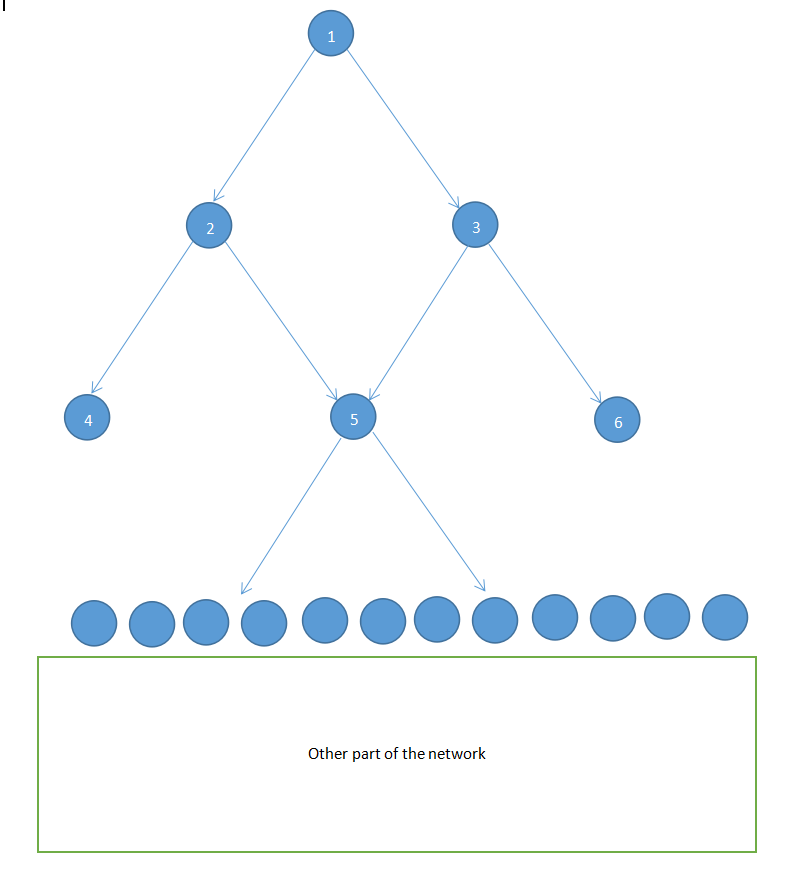
\includegraphics[width = 7cm]{1.png}
		\caption{Example network before removing $node_5$  }
		\label{fig:figure1}
	\end{figure}

	\begin{figure}[htp]
	\centering 
	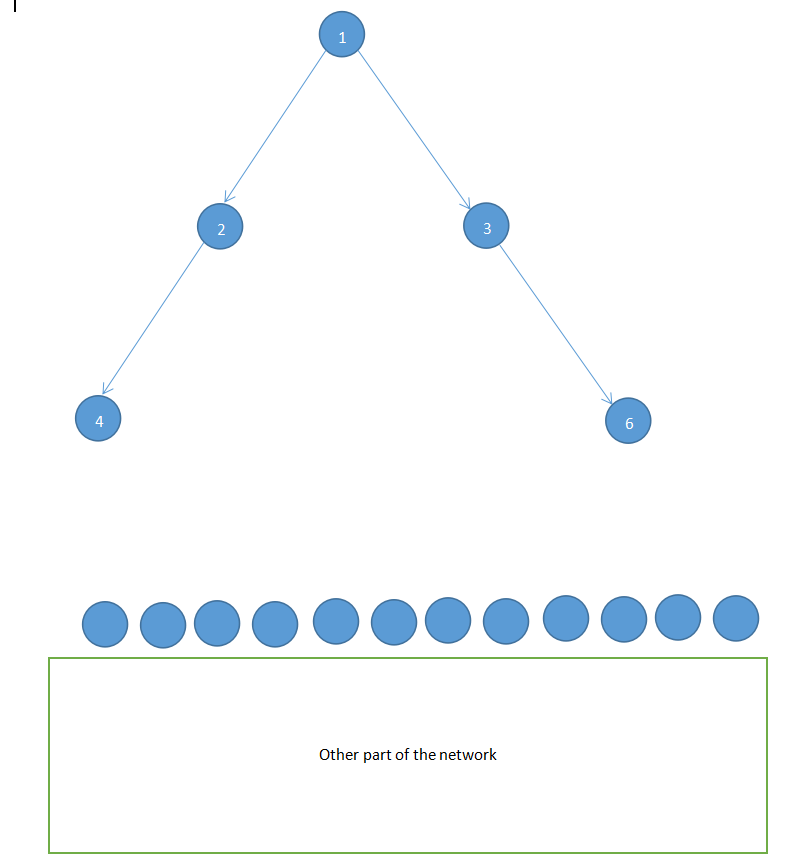
\includegraphics[width = 7cm]{2.png}
	\caption{Example network before after removing $node_5$  }
	\label{fig:figure2}
	\end{figure}
	
	
	For the network in the Figure \ref{fig:figure1}, I assume that ball radius is 1 and the next candidate removed node is $node_5$. Before the removal, CI value of $node_1$ is $((3-1)+(3-1))*(2-1)=4$. After removal in Figure \ref{fig:figure2}, it will be changed to $((2-1)+(2-1))*(2-1)=2$. However, if we follow the saying of decreasing simply by the amount $k − 1$ for the ball radius $l + 1$ (here is 2), CI value of node 1 will be $4-(k-1)=4-(2-1)=3$ . I think \cite{morone2016collective} made this mistake because they might assume there is only one shortest path from $l + 1$ node to the removed node. In fact, from the example we can see that such assumption is not correct, there are 2 shortest paths from $node_1$ to $node 5$ ($node_1$ ,$node_2$ ,$node_5$ and $node_1$ ,$node_3$ ,$node_5$). Fortunately, after scanning their provided code CI\_HEAP, I find that they didn\textquotesingle t use this concept in their implementation and still calculated the CI value of $l + 1$ node in the original formula.
	
	This section also describes the experiment on the ComplexCi and CI\_HEAP. Radius of 0,1,2 as input parameters in table \ref{tab:table6} and table \ref{tab:table7} are used to verify the performance on 8 competition datasets both for my c++ implementation ComplexCi and original c code CI\_HEAP. The \textit{minPoint} and \textit{algoEndsPoint} row are also involved into the result to evaluate the performance as brief reference. \textit{minPoint} means the number of removed nodes when ratio of giant component is invoking reinsertion on 1\%. \textit{algoEndsPoint} means the number of removed nodes when ratio of giant component is on 0. \textit{a.k.a.} there is no edge left in the network.
	
		
	
	\begin{table}[]
		\begin{adjustwidth}{-1cm}{}		
		\begin{threeparttable}		
		\centering
		\caption{Using ComplexCi to get robustness value, time, minPoint and algoEndsPoint after applying CI on 8 competition datasets with reinsertion}
		\label{tab:table6}
		\begin{tabular}{|c|c|c|c|c|c|c|c|c|c|}
			\hline
			\textbf{Radius 0} & \textbf{model1} & \textbf{model2} & \textbf{model3} & \textbf{model4} & \textbf{real1} & \textbf{real2} & \textbf{real3} & \textbf{real4} & \textbf{total} \\ \hline
			Robustness score                   & 0.2130          & 0.1783          & 0.3488          & 0.1304          & 0.0459         & 0.0918         & 0.1030         & 0.0751         & 1.1863         \\ \hline
			time                    & 150s            & 117s            & 215s            & 92s             & 203s           & 90s            & 171s           & 148s           & 215s           \\ \hline
			minPoint                & 322306          & 281709          & 538703          & 200339          & 220297         & 508819         & 93807          & 171159         &                \\ \hline
			algoEndsPoint           & 583934          & 573704          & 719722          & 534504          & 529690         & 1054742        & 151903         & 343549         &                \\ \hline
			
			\textbf{Radius 1} & \textbf{model1} & \textbf{model2} & \textbf{model3} & \textbf{model4} & \textbf{real1} & \textbf{real2} & \textbf{real3} & \textbf{real4} & \textbf{total} \\ \hline
			Robustness score                            & 0.2079          & 0.1729          & 0.3459          & 0.1258          & 0.0407         & 0.0545         & 0.0969         & 0.0654         & 1.1099         \\ \hline
			time                             & 218s            & 176s            & 324s            & 138s            & 526s           & 62s            & 637s           & 170s           & 637s           \\ \hline
			minPoint                         & 301512          & 260039          & 528727          & 190322          & 186405         & 332689         & 85279          & 162601         &                \\ \hline
			algoEndsPoint                    & 675627          & 677816          & 779027          & 632197          & 718846         & 1293988        & 186872         & 430115         &                \\ \hline		
			
			\textbf{Radius 2} & \textbf{model1} & \textbf{model2} & \textbf{model3} & \textbf{model4} & \textbf{real1} & \textbf{real2} & \textbf{real3} & \textbf{real4} & \textbf{total} \\ \hline
			Robustness score                 & 0.2083          & 0.1732          & 0.3446          & 0.1189          & 0.0387         & 0.0417         & 0.0955         & 0.0492         & 1.0701         \\ \hline
			time                             & 1757s           & 716s            & 1734s           & 475s            & 27555s         & 57s            & 43181s         & 1005s          & 43181s         \\ \hline
			minPoint                         & 301512          & 260039          & 518751          & 170288          & 169459         & 254409         & 85279          & 171159         &                \\ \hline
			algoEndsPoint                    & 686650          & 695091          & 772235          & 690491          & 766671         & 1355969        & 189648         & 509904         &                \\ \hline
	
		\end{tabular}
		\begin{tablenotes}
			\small
			\item\textit{Datasets are all verified in concurrent on the 4-core CPU machine (Intel Xeon E5-2667v4 Broadwell 3.2 GHz). The time doesn\textquotesingle t cover IO read/write from/to disk.}
		\end{tablenotes}			
		\end{threeparttable}
		\end{adjustwidth}	
	\end{table}
	
	
	\begin{table}[]
	\begin{adjustwidth}{-1cm}{}		
		\begin{threeparttable}		
			\centering
			\caption{Using CI\_HEAP to get robustness value, time, minPoint after applying CI on 8 competition datasets with reinsertion}
			\label{tab:table7}
			\begin{tabular}{|c|c|c|c|c|c|c|c|c|c|}
				\hline
				\textbf{Radius 0} & \textbf{model1} & \textbf{model2} & \textbf{model3} & \textbf{model4} & \textbf{real1} & \textbf{real2} & \textbf{real3} & \textbf{real4} & \textbf{total} \\ \hline
				Robustness score                 & 0.2121          & 0.1771          & 0.3485          & 0.1286          & 0.0450         & 0.0903         & 0.1022         & 0.0755         & 1.1793         \\ \hline
				time                             & 184s            & 156s            & 307s            & 117s            & 708s           & 95s            & 498s           & 169s           & 708s           \\ \hline
				minPoint                         & 322308          & 281711          & 538705          & 200341          & 220299         & 430541         & 93809          & 171161         &                \\ \hline
				
				\textbf{Radius 1} & \textbf{model1} & \textbf{model2} & \textbf{model3} & \textbf{model4} & \textbf{real1} & \textbf{real2} & \textbf{real3} & \textbf{real4} & \textbf{total} \\ \hline
				Robustness score                 & 0.2080          & 0.1732          & 0.3460          & 0.1249          & 0.0410         & 0.0490         & 0.0964         & 0.0659         & 1.1045         \\ \hline
				time                             & 195s            & 159s            & 333s            & 119s            & 604s           & 68s            & 727s           & 179s           & 727s           \\ \hline
				minPoint                         & 301514          & 260041          & 528729          & 190324          & 186407         & 293551         & 89545          & 162603         &                \\ \hline
				
				\textbf{Radius 2} & \textbf{model1} & \textbf{model2} & \textbf{model3} & \textbf{model4} & \textbf{real1} & \textbf{real2} & \textbf{real3} & \textbf{real4} & \textbf{total} \\ \hline
				Robustness score                 & 0.2079&0.1732&0.3446&0.1189&0.0389&0.0418&0.0955&0.0489&1.0696         \\ \hline
				time                             &  1489s&503s&1417s&316s&30771s&57s&75332s&945s&75332s
				         \\ \hline
				minPoint                         & 301514&260041&518753&170290&169461&234841&85281&171161
				     &                \\ \hline				
			\end{tabular}
			\begin{tablenotes}
				\small
				\item\textit{Datasets are all verified in concurrent on the 4-core CPU machine (Intel Xeon E5-2667v4 Broadwell 3.2 GHz). The time doesn\textquotesingle t cover IO read/write from/to disk.}
			\end{tablenotes}			
		\end{threeparttable}
		\end{adjustwidth}	
	\end{table}	
	
	It is also curious about the roles of reinsertion plays in the overall performance. What will performance of the result be if we remove the reinsertion in the algorithm of CI ? I also try to verify the case of disabling reinsertion. Results without reinsertion are shown in the table \ref{tab:table8} and table \ref{tab:table9} 
	
	\begin{table}[]
	\begin{adjustwidth}{-1cm}{}		
		\begin{threeparttable}		
			\centering
			\caption{Using ComplexCi to get robustness value, time, minPoint and algoEndsPoint after applying CI on 8 competition datasets without reinsertion}
			\label{tab:table8}
			\begin{tabular}{|c|c|c|c|c|c|c|c|c|c|}
				\hline
				\textbf{Radius 0} & \textbf{model1} & \textbf{model2} & \textbf{model3} & \textbf{model4} & \textbf{real1} & \textbf{real2} & \textbf{real3} & \textbf{real4} & \textbf{total} \\ \hline
				Robustness score                 & 0.2279          & 0.1914          & 0.3794          & 0.1446          & 0.0493         & 0.0689         & 0.1102         & 0.0922         & 1.2638         \\ \hline
				time                             & 21s             & 16s             & 20s             & 14s             & 20s            & 5s             & 19s            & 19s            & 20s            \\ \hline
				minPoint                & 322306          & 281709          & 538703          & 200339          & 220297         & 508819         & 93807          & 171159         &                \\ \hline
				algoEndsPoint           & 583934          & 573704          & 719722          & 534504          & 529690         & 1054742        & 151903         & 343549         &                \\ \hline
				
				\textbf{Radius 1} & \textbf{model1} & \textbf{model2} & \textbf{model3} & \textbf{model4} & \textbf{real1} & \textbf{real2} & \textbf{real3} & \textbf{real4} & \textbf{total} \\ \hline
				Robustness score                 & 0.2253          & 0.1878          & 0.3809          & 0.1434          & 0.0523         & 0.1069         & 0.1118         & 0.1024         & 1.3108         \\ \hline
				time                             & 115s            & 87s             & 134s            & 65s             & 359s           & 12s            & 470s           & 59s            & 470s           \\ \hline
				minPoint                         & 301512          & 260039          & 528727          & 190322          & 186405         & 332689         & 85279          & 162601         &                \\ \hline
				algoEndsPoint                    & 675627          & 677816          & 779027          & 632197          & 718846         & 1293988        & 186872         & 430115         &                \\ \hline		
				
				\textbf{Radius 2} & \textbf{model1} & \textbf{model2} & \textbf{model3} & \textbf{model4} & \textbf{real1} & \textbf{real2} & \textbf{real3} & \textbf{real4} & \textbf{total} \\ \hline
				Robustness score                 & 0.2239          & 0.1867          & 0.3777          & 0.1317          & 0.0482         & 0.0941         & 0.1085         & 0.0962         & 1.2671         \\ \hline
				time                             & 1717s           & 661s            & 1533s           & 441s            & 27250s         & 21s            & 43127s         & 907s           & 43127s         \\ \hline
				minPoint                         & 301512          & 260039          & 518751          & 170288          & 169459         & 254409         & 85279          & 171159         &                \\ \hline
				algoEndsPoint                    & 686650          & 695091          & 772235          & 690491          & 766671         & 1355969        & 189648         & 509904         &                \\ \hline
				
			\end{tabular}
			\begin{tablenotes}
				\small
				\item\textit{Datasets are all verified in concurrent on the 4-core CPU machine (Intel Xeon E5-2667v4 Broadwell 3.2 GHz). The time doesn\textquotesingle t cover IO read/write from/to disk.}
				\end{tablenotes}			
			\end{threeparttable}
		\end{adjustwidth}	
	\end{table}
	
	
	\begin{table}[]
		\begin{adjustwidth}{-1cm}{}		
			\begin{threeparttable}		
				\centering
				\caption{Using CI\_HEAP to get robustness value, time, minPoint after applying CI on 8 competition datasets without reinsertion}
				\label{tab:table9}
				\begin{tabular}{|c|c|c|c|c|c|c|c|c|c|}
					\hline
					\textbf{Radius 0} & \textbf{model1} & \textbf{model2} & \textbf{model3} & \textbf{model4} & \textbf{real1} & \textbf{real2} & \textbf{real3} & \textbf{real4} & \textbf{total} \\ \hline
					Robustness score                 & 0.2282          & 0.1916          & 0.3794          & 0.1438          & 0.0492         & 0.0773         & 0.1102         & 0.0927         & 1.2723         \\ \hline
					time                             & 18s             & 16s             & 24s             & 14s             & 22s            & 13s            & 21s            & 16s            & 22s            \\ \hline
					minPoint                         & 322308          & 281711          & 538705          & 200341          & 220299         & 430541         & 93809          & 171161         &                \\ \hline
					
					\textbf{Radius 1} & \textbf{model1} & \textbf{model2} & \textbf{model3} & \textbf{model4} & \textbf{real1} & \textbf{real2} & \textbf{real3} & \textbf{real4} & \textbf{total} \\ \hline
					Robustness score                 & 0.2254          & 0.1878          & 0.3811          & 0.1433          & 0.0533         & 0.1111         & 0.1119         & 0.1032         & 1.3170         \\ \hline
					time                             & 38s             & 27s             & 51s             & 20s             & 122s           & 12s            & 269s           & 27s            & 269s           \\ \hline
					minPoint                         & 301514          & 260041          & 528729          & 190324          & 186407         & 293551         & 89545          & 162603         &                \\ \hline
					
					\textbf{Radius 2} & \textbf{model1} & \textbf{model2} & \textbf{model3} & \textbf{model4} & \textbf{real1} & \textbf{real2} & \textbf{real3} & \textbf{real4} & \textbf{total} \\ \hline
					Robustness score                 & 0.2239          & 0.1867          & 0.3777          & 0.1317          & 0.0491         & 0.0966         & 0.1086         & 0.0965         & 1.2709         \\ \hline
					time                             & 1324s           & 384s            & 1141s           & 225s            & 30390s         & 15s            & 75070s         & 841s           & 75070s         \\ \hline
					minPoint                         & 301514          & 260041          & 518753          & 170290          & 169461         & 234841         & 85281          & 171161         &                \\ \hline				
				\end{tabular}
				\begin{tablenotes}
					\small
					\item\textit{Datasets are all verified in concurrent on the 4-core CPU machine (Intel Xeon E5-2667v4 Broadwell 3.2 GHz). The time doesn\textquotesingle t cover IO read/write from/to disk.}
				\end{tablenotes}			
			\end{threeparttable}
		\end{adjustwidth}	
	\end{table}	



	In \ref{tab:table10} and \ref{tab:table11}, the cases of "CI with reinsertion time", "CI without reinsertion time" and "reinsertion time excluding CI" are shown for ComplexCi and CI\_HEAP.

	\begin{table}[]
	\begin{adjustwidth}{-1cm}{}		
		\begin{threeparttable}		
			\centering
			\caption{Using ComplexCi to get time on 8 competition datasets, including CI with reinsertion, without reinsertion and reinsertion excluding CI}
			\label{tab:table10}
			\begin{tabular}{|c|c|c|c|c|c|c|c|c|c|}
				\hline
				\textbf{Radius 0} & \textbf{model1} & \textbf{model2} & \textbf{model3} & \textbf{model4} & \textbf{real1} & \textbf{real2} & \textbf{real3} & \textbf{real4} & \textbf{total} \\ \hline
				
				CI with reinsertion time                 & 150s&117s&215s&92s&203s&90s&171s&148s&215s         \\ \hline
				CI without reinsertion time                             & 21s&16s&20s&14s&20s&5s&19s&19s&20s            \\ \hline
				reinsertion time excluding CI                         & 129s&101s&195s&78s&183s&85s&152s&129s&195s               \\ \hline
				
				\textbf{Radius 1} & \textbf{model1} & \textbf{model2} & \textbf{model3} & \textbf{model4} & \textbf{real1} & \textbf{real2} & \textbf{real3} & \textbf{real4} & \textbf{total} \\ \hline
				
				CI with reinsertion time                 & 218s&176s&324s&138s&526s&62s&637s&170s&637s         \\ \hline
				CI without reinsertion time                             & 115s&87s&134s&65s&359s&12s&470s&59s&470s            \\ \hline
				reinsertion time excluding CI                         & 103s&89s&190s&73s&167s&50s&167s&111s&167s               \\ \hline					
				
				\textbf{Radius 2} & \textbf{model1} & \textbf{model2} & \textbf{model3} & \textbf{model4} & \textbf{real1} & \textbf{real2} & \textbf{real3} & \textbf{real4} & \textbf{total} \\ \hline
				CI with reinsertion time                 & 1757s&716s&1734s&475s&27555s&57s&43181s&1005s&43181s         \\ \hline
				CI without reinsertion time                             & 1717s&661s&1533s&441s&27250s&21s&43127s&907s&43127s         \\ \hline
				reinsertion time excluding CI                         & 40s&55s&201s&34s&305s&36s&54s&98s&54s                \\ \hline				
			\end{tabular}
			\begin{tablenotes}
				\small
				\item\textit{Datasets are all verified in concurrent on the 4-core CPU machine (Intel Xeon E5-2667v4 Broadwell 3.2 GHz). The time doesn\textquotesingle t cover IO read/write from/to disk.}
			\end{tablenotes}			
		\end{threeparttable}
	\end{adjustwidth}	
	\end{table}	


	\begin{table}[]
	\begin{adjustwidth}{-1cm}{}		
		\begin{threeparttable}		
			\centering
			\caption{Using CI\_HEAP to get time on 8 competition datasets, including CI with reinsertion, without reinsertion and reinsertion excluding CI}
			\label{tab:table11}
			\begin{tabular}{|c|c|c|c|c|c|c|c|c|c|}
				\hline
				\textbf{Radius 0} & \textbf{model1} & \textbf{model2} & \textbf{model3} & \textbf{model4} & \textbf{real1} & \textbf{real2} & \textbf{real3} & \textbf{real4} & \textbf{total} \\ \hline
				
				CI with reinsertion time                 & 1184s&156s&307s&117s&708s&95s&498s&169s&708s         \\ \hline
				CI without reinsertion time                             & 18s&16s&24s&14s&22s&13s&21s&16s&22s            \\ \hline
				reinsertion time excluding CI                         & 166s&140s&283s&103s&686s&82s&477s&153s&686s               \\ \hline
				
				\textbf{Radius 1} & \textbf{model1} & \textbf{model2} & \textbf{model3} & \textbf{model4} & \textbf{real1} & \textbf{real2} & \textbf{real3} & \textbf{real4} & \textbf{total} \\ \hline
				
				CI with reinsertion time                 & 195s&159s&333s&119s&604s&68s&727s&179s&727s         \\ \hline
				CI without reinsertion time                             & 38s&27s&51s&20s&122s&12s&269s&27s&269s            \\ \hline
				reinsertion time excluding CI                         & 157s&132s&282s&99s&482s&56s&458s&152s&458s               \\ \hline					
				
				\textbf{Radius 2} & \textbf{model1} & \textbf{model2} & \textbf{model3} & \textbf{model4} & \textbf{real1} & \textbf{real2} & \textbf{real3} & \textbf{real4} & \textbf{total} \\ \hline
				CI with reinsertion time                 & 1489s&503s&1417s&316s&30771s&57s&75332s&945s&75332s         \\ \hline
				CI without reinsertion time                             & 1324s&384s&1141s&225s&30390s&15s&75070s&841s&75070s         \\ \hline
				reinsertion time excluding CI                         & 165s&119s&276s&91s&381s&42s&262s&104s&262s                \\ \hline				
			\end{tabular}
			\begin{tablenotes}
				\small
				\item\textit{Datasets are all verified in concurrent on the 4-core CPU machine (Intel Xeon E5-2667v4 Broadwell 3.2 GHz). The time doesn\textquotesingle t cover IO read/write from/to disk.}
			\end{tablenotes}			
		\end{threeparttable}
	\end{adjustwidth}	
	\end{table}	

	
	From the experiments in table \ref{tab:table6}, \ref{tab:table7}, \ref{tab:table8}, \ref{tab:table9} , we can observe that:
	
	\begin{enumerate}
		
		
	\begin{item}
		CI in higher radius parameter performs better than Betweenness, Closeness, PageRank and Degree
	\end{item}		
		
		\begin{item}
			ComplexCi and CI\_HEAP are able to get the nearly same result in the same internal parameter. But there is still slightly different between them. I think it may be caused by the following reasons:
			
			\begin{enumerate}
				\begin{item}
					When CI removes the nodes one by one, there is the possibility that at least 2 nodes get the same CI value. CI will treat the same score nodes as the equality and choose one random node to delete. So CI depends heavily on the order of the removed node. The different deletion choice for the same score node will lead to the different robustness values finally. 
				\end{item}
				\begin{item}
					When reinsertion adds back the node one by one or a finite fraction of nodes in the batch operation, it will also meet with the same score for several nodes, which is similar with the above situation. Reinsertion will add back nodes of the same score randomly. Different reinsertion choice for the same score node will lead to the different robustness values finally as well.
				\end{item}		
				\begin{item}
					CI\_HEAP stops running algorithm when reaching \textit{minPoint} 0.01. ComplexCi will continue to run until reaching \textit{algoEndsPoint}, which represents that there is no edge in the network
				\end{item}			
				
			\end{enumerate}			
			
			
		\end{item}			
		
		\begin{item}
			Consuming time is increasing according to the higher ball radius in both ComplexCi and CI\_HEAP. After debugging and profiling, I find that most time-consuming section is to find the nodes in the scope of defined radius by using breadth-first-search (BFS) algorithm. We can not ignore BFS complexity if ball radius is high. It is also interesting that running time of CI algorithm is not related with the node number. The largest network real2 performs the quickest to complete among all datasets and the smallest real3 performs the slowest as the radius 2.
		\end{item}

	
		\begin{item}
			ComplexCI can get better speed than CI\_HEAP without reinsertion in high radius. For the real1 and real3, it can even reduce the spent time in 50\% when radius is 2. I believe the main cause is the implementation of the breadth-first-search (BFS) algorithm because it is the most time-consuming method in CI algorithm after profiling and debugging the code, though I didn\textquotesingle t get the detailed experiment statistic on it. 	
		\end{item}	
	
		\begin{item}	
			ComplexCI is better in speed in the process of reinsertion excluding CI. Using disjoint-set strategy in ComplexCi performs more efficiently than original reinsertion algorithm in CI\_HEAP.
		\end{item}	
	
		\begin{item}	
			Although the \textit{minPoint} reaches 0.01 and \textit{algoEndsPoint} reaches 0 of giant graph connected component ratio earlier in the higher radius, it seems that CI performs worse in terms of robustness value without reinsertion. I regard CI is just able to deal with controlling minimum number of nodes leading to the collapsed network, but CI is not good at getting better robustness value . So from this observation we are curious that whether the CI just works because of the reinsertion. Or can we develop the better reinsertion algorithm without using CI in robustness ? I will elaborate my thinking and experiments on that in the next chapter.	
		\end{item}		
		
	\end{enumerate}
			
	\subsection{Definitions}
	\label{definitions}
	\begin{description}
		\item[Stoichiometry]
		The relationship between the relative quantities of substances taking part in a reaction or forming a compound, typically a ratio of whole integers.
		\item[Atomic mass]
		The mass of an atom of a chemical element expressed in atomic mass units. It is approximately equivalent to the number of protons and neutrons in the atom (the mass number) or to the average number allowing for the relative abundances of different isotopes. 
	\end{description} 
	
	%----------------------------------------------------------------------------------------
	%	SECTION 2
	%----------------------------------------------------------------------------------------
	
	\section{Experimental Data}
	
	\begin{tabular}{ll}
		Mass of empty crucible & \SI{7.28}{\gram}\\
		Mass of crucible and magnesium before heating & \SI{8.59}{\gram}\\
		Mass of crucible and magnesium oxide after heating & \SI{9.46}{\gram}\\
		Balance used & \#4\\
		Magnesium from sample bottle & \#1
	\end{tabular}
	
	%----------------------------------------------------------------------------------------
	%	SECTION 3
	%----------------------------------------------------------------------------------------
	
	\section{Sample Calculation}
	
	\begin{tabular}{ll}
		Mass of magnesium metal & = \SI{8.59}{\gram} - \SI{7.28}{\gram}\\
		& = \SI{1.31}{\gram}\\
		Mass of magnesium oxide & = \SI{9.46}{\gram} - \SI{7.28}{\gram}\\
		& = \SI{2.18}{\gram}\\
		Mass of oxygen & = \SI{2.18}{\gram} - \SI{1.31}{\gram}\\
		& = \SI{0.87}{\gram}
	\end{tabular}
	
%	Because of this reaction, the required ratio is the atomic weight of magnesium: \SI{16.00}{\gram} of oxygen as experimental mass of Mg: experimental mass of oxygen or $\frac{x}{1.31}=\frac{16}{0.87}$ from which, $M_{\ce{Mg}} = 16.00 \times \frac{1.31}{0.87} = 24.1 = \SI{24}{\gram\per\mole}$ (to two significant figures).
	
	%----------------------------------------------------------------------------------------
	%	SECTION 4
	%----------------------------------------------------------------------------------------
	
	\section{Results and Conclusions}
	
	The atomic weight of magnesium is concluded to be \SI{24}{\gram\per\mol}, as determined by the stoichiometry of its chemical combination with oxygen. This result is in agreement with the accepted value.
	
	\begin{figure}[h]
		\begin{center}
			
\includegraphics[width=0.65\textwidth]{placeholder} % Include the image placeholder.png
			\caption{Figure caption.}
		\end{center}
	\end{figure}
	
	%----------------------------------------------------------------------------------------
	%	SECTION 5
	%----------------------------------------------------------------------------------------
	
	\section{Discussion of Experimental Uncertainty}
	
	The accepted value (periodic table) is \SI{24.3}{\gram\per\mole} \cite{Smith:2012qr}. The percentage discrepancy between the accepted value and the result obtained here is 1.3\%. Because only a single measurement was made, it is not possible to calculate an estimated standard deviation.
	
	The most obvious source of experimental uncertainty is the limited precision of the balance. Other potential sources of experimental uncertainty are: the reaction might not be complete; if not enough time was allowed for total oxidation, less than complete oxidation of the magnesium might have, in part, reacted with nitrogen in the air (incorrect reaction); the magnesium oxide might have absorbed water from the air, and thus weigh ``too much." Because the result obtained is close to the accepted value it is possible that some of these experimental uncertainties have fortuitously cancelled one another.
	
	%----------------------------------------------------------------------------------------
	%	SECTION 6
	%----------------------------------------------------------------------------------------
	
	\section{Answers to Definitions}
	
	\begin{enumerate}
		\begin{item}
			The \emph{atomic weight of an element} is the relative weight of one of its atoms compared to C-12 with a weight of 12.0000000$\ldots$, hydrogen with a weight of 1.008, to oxygen with a weight of 16.00. Atomic weight is also the average weight of all the atoms of that element as they occur in nature.
		\end{item}
		\begin{item}
			The \emph{units of atomic weight} are two-fold, with an identical numerical value. They are g/mole of atoms (or just g/mol) or amu/atom.
		\end{item}
		\begin{item}
			\emph{Percentage discrepancy} between an accepted (literature) value and an experimental value is
			\begin{equation*}
				\frac{\mathrm{experimental\;result} - \mathrm{accepted\;result}}{\mathrm{accepted\;result}}
			\end{equation*}
		\end{item}
	\end{enumerate}
	
	%----------------------------------------------------------------------------------------
	%	BIBLIOGRAPHY
	%----------------------------------------------------------------------------------------
	
	\bibliographystyle{abbrv}
	
	\bibliography{sample}
	
	%----------------------------------------------------------------------------------------
	
	
\end{document}